%
% This document contains the chapter about AC analysis.
%
% Copyright (C) 2003, 2004, 2005 Stefan Jahn <stefan@lkcc.org>
% Copyright (C) 2004 Michael Margraf <Michael.Margraf@alumni.TU-Berlin.DE>
%
% Permission is granted to copy, distribute and/or modify this document
% under the terms of the GNU Free Documentation License, Version 1.1
% or any later version published by the Free Software Foundation.
%

\chapter{AC Analysis}
%\addcontentsline{toc}{chapter}{AC Analysis}
\label{sec:acMNA}

The AC analysis is a small signal analysis in the frequency domain.
Basically this type of simulation uses the same algorithms as the DC
analysis (section \ref{sec:MNA} on page \pageref{sec:MNA}).  The AC
analysis is a linear modified nodal analysis.  Thus no iterative
process is necessary.  With the Y-matrix of the components, i.e. now a
complex matrix, and the appropriate extensions it is necessary to
solve the equation system \eqref{eq:acMNA} similar to the (linear) DC
analysis.
\begin{equation}
\label{eq:acMNA}
\left[A\right] \cdot \left[x\right] = \left[z\right]
\;\;\;\; \textrm{ with } \;\;\;\;
A =
\begin{bmatrix}
Y & B\\
C & D
\end{bmatrix}
\end{equation}

\section{MNA matrix entries of reactive components}
%\addcontentsline{toc}{section}{MNA matrix entries of reactive components}

If not otherwise noted the MNA matrix elements and the extensions of
the components (section \ref{sec:MNAext} on page \pageref{sec:MNAext})
for the AC analysis do not differ from those for the DC analysis.  The
Y-matrices of the non-linear devices and certain microstrip components
are documented in the appropriate sections (see chapter
\ref{sec:NLdevices} and \ref{sec:MScomponents}).

\subsection{Capacitor}
%\addcontentsline{toc}{subsection}{Capacitor}

The Y-parameter matrix of an ideal capacitor with the capacitance $C$
writes as follows.
\begin{equation}
Y =
\begin{bmatrix}
+j\omega C & -j\omega C\\
-j\omega C & +j\omega C\\
\end{bmatrix}
\end{equation}

\subsection{Inductor}
%\addcontentsline{toc}{subsection}{Inductor}

The Y-parameter matrix of an ideal inductor with the inductance $L$
writes as follows.
\begin{equation}
Y =
\begin{bmatrix}
+\dfrac{1}{j\omega L} & -\dfrac{1}{j\omega L}\\
-\dfrac{1}{j\omega L} & +\dfrac{1}{j\omega L}\\
\end{bmatrix}
\end{equation}

\subsection{Transmission line}
%\addcontentsline{toc}{subsection}{Transmission line}
\label{sec:tl_yparameter}

A transmission line is usually described by its ABCD-matrix.  (Note
that in ABCD-matrices, i.e. the chain matrix representation, the
current $i_2$ is defined to flow out of the output port.)
\begin{equation}
\left(\underline{A}\right) =
\begin{pmatrix}
\cosh{\left(\gamma\cdot l\right)} & Z_L\cdot \sinh{\left(\gamma\cdot l\right)}\\
\sinh{\left(\gamma\cdot l\right)} / Z_L & \cosh{\left(\gamma\cdot l\right)}
\end{pmatrix}
\end{equation}

These can easily be recalculated into impedance parameters.
\begin{align}
Z_{11} = Z_{22} &= \frac{Z_L}{\tanh{\left(\gamma\cdot l\right)}}\\
Z_{12} = Z_{21} &= \frac{Z_L}{\sinh{\left(\gamma\cdot l\right)}}
\end{align}

Or in admittance parameter representation it yields
\begin{equation}
\label{eq:TransLineY}
\begin{split}
Y_{11} = Y_{22} &= \frac{1}{Z_L \cdot \tanh{\left(\gamma\cdot l\right)}}\\
Y_{12} = Y_{21} &= \frac{-1}{Z_L\cdot \sinh{\left(\gamma\cdot l\right)}}
\end{split}
\end{equation}

whence $\gamma$ denotes the propagation constant $\alpha + j\beta$ and
$l$ is the length of the transmission line.  $Z_L$ represents the
characteristic impedance of the transmission line.  The Y-parameters
as defined by eq. \eqref{eq:TransLineY} can be used for the microstrip
line.  For an ideal, i.e. lossless, transmission lines they write
accordingly.
\begin{align}
Z_{11} = Z_{22} &= \frac{Z_L}{j\cdot\tan{\left(\beta\cdot l\right)}}\\
Z_{12} = Z_{21} &= \frac{Z_L}{j\cdot\sin{\left(\beta\cdot l\right)}}\\
Y_{11} = Y_{22} &= \frac{1}{j\cdot Z_L \cdot \tan{\left(\beta\cdot l\right)}}\\
Y_{12} = Y_{21} &= \frac{j}{Z_L\cdot \sin{\left(\beta\cdot l\right)}}
\end{align}

\subsection{Coupled transmission line}
%\addcontentsline{toc}{subsection}{Coupled transmission line}

A coupled transmission line is described by two identical transmission
line ABCD-matrices, one for the even and one for the odd mode.
Because the coupled lines are a symmetrical 3-line system, the
matrices are completely independent of each other.  Therefore, its
Y-parameters write as follows.
\begin{align}
Y_{11} = Y_{22} = Y_{33} = Y_{44} &= \frac{1}{2\cdot Z_{L,e} \cdot \tanh\left(\gamma_e\cdot l\right)}
              + \frac{1}{2\cdot Z_{L,o} \cdot \tanh\left(\gamma_o\cdot l\right)}\\
Y_{12} = Y_{21} = Y_{34} = Y_{43} &= \frac{-1}{2\cdot Z_{L,e} \cdot \sinh\left(\gamma_e\cdot l\right)}
              + \frac{-1}{2\cdot Z_{L,o} \cdot \sinh\left(\gamma_o\cdot l\right)}\\
Y_{13} = Y_{31} = Y_{24} = Y_{42} &= \frac{-1}{2\cdot Z_{L,e} \cdot \sinh\left(\gamma_e\cdot l\right)}
              + \frac{1}{2\cdot Z_{L,o} \cdot \sinh\left(\gamma_o\cdot l\right)}\\
Y_{14} = Y_{41} = Y_{23} = Y_{32} &= \frac{1}{2\cdot Z_{L,e} \cdot \tanh\left(\gamma_e\cdot l\right)}
              + \frac{-1}{2\cdot Z_{L,o} \cdot \tanh\left(\gamma_o\cdot l\right)}
\end{align}

\subsection{Phase shifter}
%\addcontentsline{toc}{subsection}{Phase shifter}

A phase shifter is no more than an ideal transmission line with a
negative length and its Z-parameters write as follows.
\begin{align}
Z_{11} = Z_{22} &= \frac{j\cdot Z_{ref}}{\tan(\phi)}\\
Z_{12} = Z_{21} &= \frac{j\cdot Z_{ref}}{\sin(\phi)}
\end{align}

The admittance parameters required for the AC analysis result in
\begin{align}
Y_{11} = Y_{22} &= \frac{1}{j\cdot Z_{ref} \cdot \tan{\left(\phi\right)}}\\
Y_{12} = Y_{21} &= \frac{j}{Z_{ref}\cdot \sin{\left(\phi\right)}}
\end{align}

where $\phi$ denotes the actual phase shift of the device.  For a zero
phase shift ($\phi = 0$) neither the Z- nor the Y-parameters are
defined.  That is why during AC analysis a phase shifter with zero
phase shift represents an ideal short circuit regardless its reference
impedance.

\addvspace{12pt}

The MNA matrix entries of an ideal short circuit during AC and DC
analysis correspond to a voltage source with zero voltage.  The
complete MNA matrix representation writes as follows
\begin{equation}
\begin{bmatrix}
. & . & +1\\
. & . & -1\\
+1 & -1 & 0\\
\end{bmatrix}
\cdot
\begin{bmatrix}
V_1\\
V_2\\
I_{br}\\
\end{bmatrix}
=
\begin{bmatrix}
I_1\\
I_2\\
0
\end{bmatrix}
\end{equation}

whence $I_{br}$ denote the branch current through the voltage source.

\subsection{Attenuator}
%\addcontentsline{toc}{subsection}{Attenuator}

The impedance parameters of an attenuator with the power attenuation
$L$ (loss) (or power gain $G=1/L$) in reference to the impedance
$Z_{ref}$ write as follows.
\begin{align}
Z_{11} = Z_{22} &= Z_{ref}\cdot\frac{L+1}{L-1}\\
Z_{12} = Z_{21} &= Z_{ref}\cdot\frac{2\cdot\sqrt{L}}{L-1}
\end{align}

The Z-parameters can be easily converted into Y-parameters which are
required for the AC analysis.  An attenuator with a power attenuation
$L=1$ (no attenuation) yields an ideal short circuit regardless its
reference impedance very similar to the phase shifter with zero phase
shift.

\subsection{Controlled sources}
%\addcontentsline{toc}{subsection}{Controlled sources}

During AC analysis the transfer factors $G$ of the controlled sources
described in sections \ref{sec:vccs}, \ref{sec:vcvs}, \ref{sec:cccs}
and \ref{sec:ccvs} on page \pageref{sec:vccs} ff. result in a complex
value depending on the delay time $T$ and frequency $f$.
\begin{equation}
\underline{G} = G\cdot e^{j\omega T} = G\cdot e^{j\cdot 2\pi f\cdot T}
\end{equation}

No more changes to the MNA matrix entries are necessary in order to
use those of the DC analysis for the AC analysis.

\section{Other AC components}
%\addcontentsline{toc}{section}{Other AC components}

The following sections describe the MNA matrix entries required for
the small signal AC analysis of the remaining components not yet
discussed in previous sections.  Only components whose MNA matrix
entries differ from the DC analysis MNA entries are taken into
account.

\subsection{DC Feed and DC Block}
%\addcontentsline{toc}{subsection}{DC Feed and DC Block}

Both of the devices exchange their role in AC and DC analysis.  Thus
the MNA matrix entries of the DC feed during DC analysis correspond to
the MNA matrix entries of the DC block during AC analysis and the
other way around.

\addvspace{12pt}

During AC analysis the DC feed corresponds to an ideal open circuit
with the MNA matrix entries
\begin{equation}
\begin{bmatrix}
. & .\\
. & .\\
\end{bmatrix}
\cdot
\begin{bmatrix}
V_1\\
V_2\\
\end{bmatrix}
=
\begin{bmatrix}
I_1\\
I_2\\
\end{bmatrix}
\end{equation}

The MNA matrix entries of a DC block correspond to an ideal short
circuit during AC analysis which is modeled by a voltage source with
zero voltage.
\begin{equation}
\begin{bmatrix}
. & . & +1\\
. & . & -1\\
+1 & -1 & 0\\
\end{bmatrix}
\cdot
\begin{bmatrix}
V_1\\
V_2\\
I_{br}\\
\end{bmatrix}
=
\begin{bmatrix}
I_1\\
I_2\\
0
\end{bmatrix}
\end{equation}

\subsection{Bias T}
%\addcontentsline{toc}{subsection}{Bias T}

Figure \ref{fig:ACbiast} denotes a combination of DC feed and DC
block.  During AC analysis node 1 and 3 simply exchange their roles in
comparison to the DC analysis.

\begin{figure}[ht]
\begin{center}
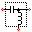
\includegraphics[width=3.5cm]{biast}
\end{center}
\caption{bias t}
\label{fig:ACbiast}
\end{figure}
\FloatBarrier

Using the port configuration shown in fig. \ref{fig:ACbiast} the
complete MNA entries of the bias t during AC analysis write as
follows.
\begin{equation}
\begin{bmatrix}
 . & . & .  & -1\\
 . & . & .  &  1\\
 . & . & .  &  0\\
-1 & 1 & 0  &  0
\end{bmatrix}
\cdot
\begin{bmatrix}
V_{1}\\
V_{2}\\
V_{3}\\
I_{out}
\end{bmatrix}
=
\begin{bmatrix}
I_{1}\\
I_{2}\\
I_{3}\\
0
\end{bmatrix}
\end{equation}

\subsection{S-parameter container with additional reference port}
%\addcontentsline{toc}{subsection}{S-parameter container with additional reference port}

The Y-parameters of a multi-port component defined by its S-parameters
as described in section \ref{sec:spfile} of page \pageref{sec:spfile}
required for a small signal AC analysis can be obtained by converting
the S-parameters into Y-parameters.

\subsection{Non-ideal transformer}
%\addcontentsline{toc}{subsection}{Non-ideal transformer}

Many simulators support non-ideal transformers (e.g. mutual inductor
in SPICE).  An often used model consists of finite inductances and an
imperfect coupling (straw inductance).  This model has three
parameters: Inductance of the primary coil $L_1$, inductance of the
secondary coil $L_2$ and the coupling factor $k=0...1$.

\addvspace{12pt}

This model can be replaced by the equivalent circuit depicted in
figure \ref{fig:nitrafo}.  The values are calculated as follows.

\begin{align}
\textrm{turn ratio:} & \qquad  T = \sqrt{\frac{L_1}{L_2}}\\
\textrm{mutual inductance:}  & \qquad M = k\cdot L_1\\
\textrm{primary inductance:}  & \qquad L_{1,new} = L_1 - M = L_1\cdot (1-k)\\
\textrm{secondary inductance:}  & \qquad L_{2,new} = L_2 - \frac{M}{T^2} = L_2\cdot (1-k)
\end{align}

\begin{figure}[ht]
\begin{center}
\includegraphics[width=7.5cm]{nitrafo}
\end{center}
\caption{equivalent circuit of non-ideal transformer}
\label{fig:nitrafo}
\end{figure}
\FloatBarrier

The Y-parameters of this component are:
\begin{align}
Y_{11} = Y_{44} = -Y_{41} = -Y_{14} &= \frac{1}{j\omega\cdot L_1\cdot (1-k^2)}\\
Y_{22} = Y_{33} = -Y_{23} = -Y_{32} &= \frac{1}{j\omega\cdot L_2\cdot (1-k^2)}\\
Y_{13} = Y_{31} = Y_{24} = Y_{42} = -Y_{12} = -Y_{21} = -Y_{34} = -Y_{43} &=
  \frac{k}{j\omega\cdot\sqrt{L_1\cdot L_2}\cdot (1-k^2)}
\end{align}

Also including an ohmic resistance $R_1$ and $R_2$ for each coil,
leads to the following Y-parameters:
\begin{align}
Y_{11} = Y_{44} = -Y_{41} = -Y_{14} &
  = \dfrac{1}{j\omega\cdot L_1\cdot \left(1-k^2\cdot\dfrac{j\omega L_2}{j\omega L_2 + R_2}\right) + R_1}\\
Y_{22} = Y_{33} = -Y_{23} = -Y_{32} &
  = \dfrac{1}{j\omega\cdot L_2\cdot \left(1-k^2\cdot\dfrac{j\omega L_1}{j\omega L_1 + R_1}\right) + R_2}\\
Y_{13} = Y_{31} = Y_{24} = Y_{42} = -Y_{12} &= -Y_{21} = -Y_{34} = -Y_{43} =
  k\cdot\frac{j\omega\sqrt{L_1\cdot L_2}}{j\omega\cdot L_2 + R_2}\cdot Y_{11}
\end{align}

Building the S-parameters leads to too large equations. Converting
the Y-parameters into S-parameters is therefore recommended.\\
The MNA matrix entries and the noise correlation matrices
of this transformer are:
\begin{equation}
(\underline{Y}) =
\begin{pmatrix}
 1/R_1 & 0 & 0 & -1/R_1 \\
 0 &  1/R_2 & -1/R_2 & 0 \\
 0 & -1/R_2 &  1/R_2 & 0 \\
-1/R_1 & 0 & 0 &  1/R_1 \\
\end{pmatrix}
\end{equation}
\begin{equation}
(\underline{C}_Y) = 4\cdot k\cdot T\cdot
\begin{pmatrix}
 1/R_1 & 0 & 0 & -1/R_1 \\
 0 &  1/R_2 & -1/R_2 & 0 \\
 0 & -1/R_2 &  1/R_2 & 0 \\
-1/R_1 & 0 & 0 &  1/R_1 \\
\end{pmatrix}
\end{equation}
\begin{equation}
(\underline{C}_S) = 4\cdot k\cdot T\cdot Z_0\cdot
\begin{pmatrix}
 \frac{R_1}{(2\cdot Z_0 + R_1)^2} & 0 & 0 & -\frac{R_1}{(2\cdot Z_0 + R_1)^2} \\
 0 &  \frac{R_2}{(2\cdot Z_0 + R_2)^2} & -\frac{R_2}{(2\cdot Z_0 + R_2)^2} & 0 \\
 0 & -\frac{R_2}{(2\cdot Z_0 + R_2)^2} &  \frac{R_2}{(2\cdot Z_0 + R_2)^2} & 0 \\
-\frac{R_1}{(2\cdot Z_0 + R_1)^2} & 0 & 0 &  \frac{R_1}{(2\cdot Z_0 + R_1)^2} \\
\end{pmatrix}
\end{equation}


\addvspace{12pt}

A transformer with three coupled inductors has three coupling factors
$k_{12}$, $k_{13}$ and $k_{23}$.  Its Y-parameters write as follows
(port numbers are according to figure \ref{fig:symtrafo}).

\begin{gather}
A = j\omega\cdot (1 - k_{12}^2 - k_{13}^2 - k_{23}^2 + 2\cdot k_{12}\cdot k_{13}\cdot k_{23} ) \\
Y_{11} = Y_{66} = -Y_{16} = -Y_{61} = \dfrac{1-k_{23}^2}{L_1\cdot A} \\
Y_{22} = Y_{33} = -Y_{23} = -Y_{32} = \dfrac{1-k_{12}^2}{L_3\cdot A} \\
Y_{44} = Y_{55} = -Y_{45} = -Y_{54} = \dfrac{1-k_{13}^2}{L_2\cdot A} \\
Y_{12} = Y_{21} = Y_{36} = Y_{63} = -Y_{13} = -Y_{31} = -Y_{26} = -Y_{62}
   = \dfrac{k_{12}\cdot k_{23} - k_{13}}{\sqrt{L_1\cdot L_3}\cdot A} \\
Y_{15} = Y_{51} = Y_{46} = Y_{64} = -Y_{14} = -Y_{41} = -Y_{56} = -Y_{65}
   = \dfrac{k_{13}\cdot k_{23} - k_{12}}{\sqrt{L_1\cdot L_2}\cdot A} \\
Y_{25} = Y_{52} = Y_{43} = Y_{34} = -Y_{24} = -Y_{42} = -Y_{53} = -Y_{35}
   = \dfrac{k_{12}\cdot k_{13} - k_{23}}{\sqrt{L_2\cdot L_3}\cdot A}
\end{gather}
